\documentclass[pdftex,12pt,a4paper]{article}
\newcommand{\HRule}{\rule{\linewidth}{0.5mm}}


\usepackage{graphicx}
\usepackage[margin=2.75cm]{geometry}
\usepackage{tikz}
\usepackage{amsmath}
\usepackage{listings}
\usepackage{color}
\usepackage{hyperref}
\usepackage{algorithm}
\usepackage{algpseudocode}
\usepackage{lipsum}

\usetikzlibrary{decorations.pathmorphing}
\usetikzlibrary{shapes}
\tikzset{snake it/.style={decorate, decoration=snake}}
\linespread{1.3}

\makeatletter
\newenvironment{breakablealgorithm}
  {% \begin{breakablealgorithm}
   \begin{center}
     \refstepcounter{algorithm}% New algorithm
     \hrule height.8pt depth0pt \kern2pt% \@fs@pre for \@fs@ruled
     \renewcommand{\caption}[2][\relax]{% Make a new \caption
       {\raggedright\textbf{\ALG@name~\thealgorithm} ##2\par}%
       \ifx\relax##1\relax % #1 is \relax
         \addcontentsline{loa}{algorithm}{\protect\numberline{\thealgorithm}##2}%
       \else % #1 is not \relax
         \addcontentsline{loa}{algorithm}{\protect\numberline{\thealgorithm}##1}%
       \fi
       \kern2pt\hrule\kern2pt
     }
  }{% \end{breakablealgorithm}
     \kern2pt\hrule\relax% \@fs@post for \@fs@ruled
   \end{center}
  }
\makeatother


\lstdefinestyle{customc}{
  belowcaptionskip=1\baselineskip,
  breaklines=true,
  frame=L,
  xleftmargin=\parindent,
  language=C,
  showstringspaces=false,
  basicstyle=\footnotesize\ttfamily,
  keywordstyle=\bfseries\color{green!40!black},
  commentstyle=\itshape\color{purple!40!black},
  identifierstyle=\color{blue},
  stringstyle=\color{orange},
  tabsize=2,
}

\lstdefinestyle{customasm}{
  belowcaptionskip=1\baselineskip,
  frame=L,
  xleftmargin=\parindent,
  language=[x86masm]Assembler,
  basicstyle=\footnotesize\ttfamily,
  commentstyle=\itshape\color{purple!40!black},
}

\lstset{escapechar=@,style=customc}


\begin{document}



%%%%%%%%%%%%%%%%%%%%%%
%%%%% TITLE PAGE %%%%%
%%%%%%%%%%%%%%%%%%%%%%

\begin{titlepage}
\begin{center}
\pagenumbering{gobble}

\begin{figure}

\centering
\includegraphics[width=30mm]{Crest.png}

\end{figure}


\textsc{\LARGE Trinity College Dublin}\\
\textsc{\Large School of Mathematics}

\HRule \\[0.4cm]
{\huge \bfseries Spin models on random bipartite graphs \\[0.4cm] }

\HRule \\[1.5cm]

\Large \emph{Author:} \\ Shane Harding \\[0.8cm]

\large \emph{Supervisor:} \\ Prof. Mike Peardon

\end{center}

\end{titlepage}

%%%%%%%%%%%%%%%%%%%%%%



\pagenumbering{roman}
%%%%%%%%%%%%%%%%%%%%
%%%%% ABSTRACT %%%%%
%%%%%%%%%%%%%%%%%%%%



\vspace*{\fill}
\begin{abstract}

This is my abstract.

\end{abstract}
\vspace*{\fill}

\newpage

%%%%%%%%%%%%%%%%%%%%%%%%%%%%%
%%%%% TABLE OF CONTENTS %%%%%
%%%%%%%%%%%%%%%%%%%%%%%%%%%%%

\tableofcontents

\newpage
\pagenumbering{arabic}


%%%%%%%%%%%%%%%%%%%%%%%%
%%%%% INTRODUCTION %%%%%
%%%%%%%%%%%%%%%%%%%%%%%%

\section{Introduction}

This project is centered around doing Ising Model simulations on random bipartite graphs. As such, it is useful to know more the Ising model and graph theory before we get started.

%%%%% ISING MODEL %%%%%

\subsection{The Ising Model}


%%%%% WHAT IS ISING MODEL %%%%%

\subsubsection{What is the Ising Model?}

The Ising Model is a mathematical model that was invented by Wilhelm Lenz, but developed by Ernst Ising in 1925. It is used to to explore ferromagnetism in statistical physics.

\emph{Statistical physics} refers to the method by which microscopic laws of physics are used to create an understanding of Nature on a macroscopic scale. It is a branch of physics that relies on probability theory and statistics to solve physical problems with large population sizes. It is used to describe a wide spectrum of problems that are inherently stochastic.

The Ising model consists of discrete variables that represent the magnetic dipole moments of atomic spins. These are the intrinsic magnetic moments possessed by every electron and can take the values $\pm1$. A spin of $+1$ is called \emph{spin up} and represented by: $\uparrow$. While a spin of $-1$ is called \emph{spin down} and represented by $\downarrow$. The magnetic phenomena in some materials is ca
used by the quantum-mechanical ‘spin’ of electrons.

The model is usually represented on a rectangular lattice. Each lattice point represents an atom in the material and is assigned a spin value at the begining of the calculation (usually a random value assignment, but can also be an ordered assignment where all spins are initialised to spin up, say).

Considering a lattice, denoted by $\lambda$, at each lattice site $k$ there is a discrete spin value, $\sigma_k$, such that $\sigma_k \in \{-1,+1\}$. We call a spin configuration the assignment of a spin value to each of the lattice sites.

For a pair of adjacent sites $i,j$, there is the interaction $J_{ij}$. If there is an external magnetic field interacting with sit $j$ we denote it by $h_j$. The energy of a configuration $\sigma$ is given by the Hamiltonian function:

\[ H(\sigma) = - \sum_{nn(i,j)} J_{ij} \sigma_i \sigma_j - \mu \sum_{j} h_j \sigma_j \]

The first sum is for pairs of adjacent spins (each pair counted once), where the notation $nn(i,j)$ means that $i$ and $j$ are nearest neighbours. $\mu$ is the magnetic moment.

For the duration of this project we will be discussing the case with no external magnetic field, $h_j = 0$. So the Hamiltonian is simply:

\[ H(\sigma) = - \sum_{nn(i,j)} J_{ij} \sigma_i \sigma_j  \]

We will also restrict ourselves to the ferromagnetic case, where $J_{ij} > 0$. In a ferromagnetic Ising model spins seek a configuration such that they are all aligned. We will also have the same interaction for all pairs: $J_{ij} = J$

The Boltzmann distribution gives the configuration probability:

\[ P_{\beta}(\sigma) = \frac{e^{-\beta H(\sigma)}}{Z_{\beta}} \].

Where $\beta = \frac{1}{k_B T}$, the inverse of the product of the Boltzmann constant and the temperature. The normalisation constant $Z_{\beta} = \sum_{\sigma} e^{-\beta H(\sigma)}$ is the \emph{partition function}.

The partition function is of central importance in statistical physics. It describes the statistical properties of a system in thermodynamic equilibrium. Many of the thermodynamic variables of a system can be described through the partition function or its derivatives.

To update a point the Metropolis Hastings algorithm is used to update each point on the graph. To update one node, $i$, its Hamiltonian is first calculated. This is simply given by:

\[ H(\sigma_i) = \sum_{nn(ij)} \delta_{ij}, \]

where $\delta_{ij}$ is the kronecker delta: 

\[ \delta_{ij} = \left\{ \begin{array}{ll}
         1 & \mbox{if $i = j$};\\
        0 & \mbox{if $i \neq j$}.\end{array} \right. \]

Once the Hamiltonian is calculated, a spin filp for point $i$ is proposed. This involves simply flipping its current spin. So if it has spin up it gets changed to spin down and vice versa. The Hamiltonian is then calculated for this new proposed spin.

If the value of the new Hamiltonian is strictly less than that of the original Hamiltonian the proposed spin flip is accepted. If not, the proposed spin flip is accepted with probability $e^{-2 \beta (H_{new} - H_{old})}$. One `sweep' or update consists of doing this for all of the spins on the graph.

Below a certain temperature, know as the \emph{Curie temperature}, $T_C$, the spins will spontaneously align. This is know as the phase transition. It can be show that for the one dimensional Ising model there is no phase transition. It can also be shown analytically that there is a phase transition for the two dimensional lattice Ising model.


%%%%% COMPUTATION METHODS %%%%%

\subsubsection{How it is normally studied in serial and parallel simulations}

The two dimenstional Ising model is usually represented as a rectangular lattice, sometimes with periodic boundary conditions and sometimes not, depending on the case in question. Each point on the lattice is assigned a spin at the start of the simulation, usually at random. Each point only `feels' the interaction of its nearest neighbours (each point has four neighbours). These interactions allow a Hamiltonian to be calculated for each point.

In parallel we divide the grid up into smaller subgrids. In figure FILL, the grid is divided into four subgrids but obviously more subdivisions are possible. Normally we have one subgrid per processor that we intend to run the program on. The need for \emph{Message Passing Interface} (MPI) function calls arises from the fact that on the edges of our subgrids there are points needed for the update step whose values are stored on another processor. These values need to be identified and passed to the relevant processor. MPI is used for this task. The easiest method is to load all the `halo' data into a buffer and send it with MPI send from the sending process to the receiving one that calls MPI receive. This send/receive is to be done between each update step.



%%%%% REGULAR LATTICE ISING PIC %%%%%
\begin{figure}
\begin{center}
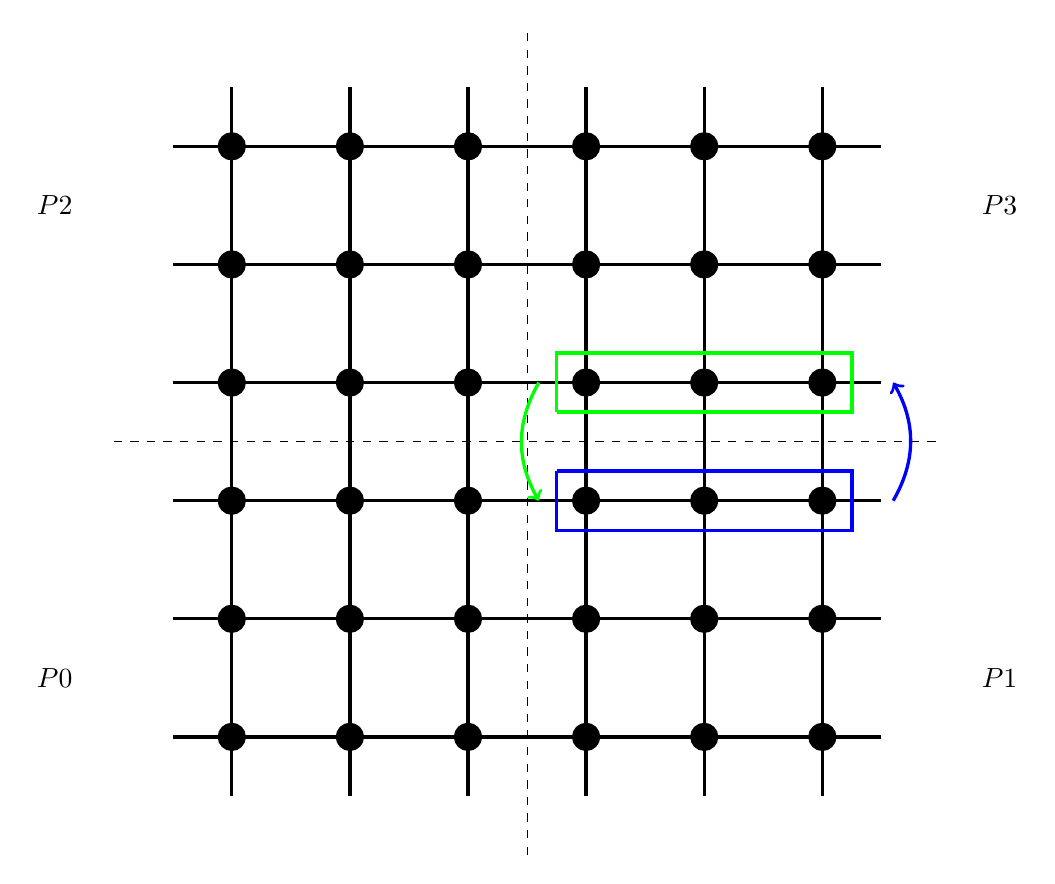
\begin{tikzpicture}[scale=1.5]

\node at (-4, -2) {$P0$};
\node at (4,-2) {$P1$};
\node at (-4, 2) {$P2$};
\node at (4,2) {$P3$};

\draw [very thick] (-3,-2.5) -- (3,-2.5);
\draw [very thick] (-3,-1.5) -- (3,-1.5);
\draw [very thick] (-3,-0.5) -- (3,-0.5);
\draw [very thick] (-3,0.5) -- (3,0.5);
\draw [very thick] (-3,1.5) -- (3,1.5);
\draw [very thick] (-3,2.5) -- (3,2.5);

\draw [dashed] (-3.5,0) -- (3.5,0);
\draw [dashed] (0,-3.5) -- (0,3.5);

\draw [very thick] (-2.5,-3) -- (-2.5,3);
\draw [very thick] (-1.5,-3) -- (-1.5,3);
\draw [very thick] (-0.5,-3) -- (-0.5,3);
\draw [very thick] (0.5,-3) -- (0.5,3);
\draw [very thick] (1.5,-3) -- (1.5,3);
\draw [very thick] (2.5,-3) -- (2.5,3);

\draw [blue,very thick] (0.25, -0.25) -- (0.25, -0.75) -- (2.75,-0.75) -- (2.75,-0.25) -- (0.25, -0.25);
\draw [->][blue, very thick] (3.1,-0.5) to [out=60,in=300] (3.1,0.5);

\draw [green,very thick] (0.25, 0.25) -- (0.25, 0.75) -- (2.75,0.75) -- (2.75,0.25) -- (0.25, 0.25);
\draw [->][green, very thick] (0.1,0.5) to [out=240,in=120] (0.1,-0.5);

\draw [fill=black,very thick] (-2.5,-2.5) circle (3pt);
\draw [fill=black,very thick] (-1.5,-2.5) circle (3pt);
\draw [fill=black,very thick] (-0.5,-2.5) circle (3pt);
\draw [fill=black,very thick] (0.5,-2.5) circle (3pt);
\draw [fill=black,very thick] (1.5,-2.5) circle (3pt);
\draw [fill=black,very thick] (2.5,-2.5) circle (3pt);

\draw [fill=black,very thick] (-2.5,-1.5) circle (3pt);
\draw [fill=black,very thick] (-1.5,-1.5) circle (3pt);
\draw [fill=black,very thick] (-0.5,-1.5) circle (3pt);
\draw [fill=black,very thick] (0.5,-1.5) circle (3pt);
\draw [fill=black,very thick] (1.5,-1.5) circle (3pt);
\draw [fill=black,very thick] (2.5,-1.5) circle (3pt);

\draw [fill=black,very thick] (-2.5,-0.5) circle (3pt);
\draw [fill=black,very thick] (-1.5,-0.5) circle (3pt);
\draw [fill=black,very thick] (-0.5,-0.5) circle (3pt);
\draw [fill=black,very thick] (0.5,-0.5) circle (3pt);
\draw [fill=black,very thick] (1.5,-0.5) circle (3pt);
\draw [fill=black,very thick] (2.5,-0.5) circle (3pt);

\draw [fill=black,very thick] (-2.5,0.5) circle (3pt);
\draw [fill=black,very thick] (-1.5,0.5) circle (3pt);
\draw [fill=black,very thick] (-0.5,0.5) circle (3pt);
\draw [fill=black,very thick] (0.5,0.5) circle (3pt);
\draw [fill=black,very thick] (1.5,0.5) circle (3pt);
\draw [fill=black,very thick] (2.5,0.5) circle (3pt);

\draw [fill=black,very thick] (-2.5,1.5) circle (3pt);
\draw [fill=black,very thick] (-1.5,1.5) circle (3pt);
\draw [fill=black,very thick] (-0.5,1.5) circle (3pt);
\draw [fill=black,very thick] (0.5,1.5) circle (3pt);
\draw [fill=black,very thick] (1.5,1.5) circle (3pt);
\draw [fill=black,very thick] (2.5,1.5) circle (3pt);

\draw [fill=black,very thick] (-2.5,2.5) circle (3pt);
\draw [fill=black,very thick] (-1.5,2.5) circle (3pt);
\draw [fill=black,very thick] (-0.5,2.5) circle (3pt);
\draw [fill=black,very thick] (0.5,2.5) circle (3pt);
\draw [fill=black,very thick] (1.5,2.5) circle (3pt);
\draw [fill=black,very thick] (2.5,2.5) circle (3pt);

\end{tikzpicture}
\caption{Regular square lattice Ising model. The nodes inside the blue rectangle show the data points on process 1 that are needed on process 3 in order to complete an update step. The green rectangle has the points on process 3 that are to be sent to process 1.}
\end{center}
\end{figure}

It is worth noting at this stage that the square latice is also a bipartite graph. It is possibl to pick a point and say that it is in set $A$, then label all four of its nearest neighbours as being in set $B$. Each of these points in B will have three other neighbours (ignoring the initial point chosen), and these three neighbours are labeled as being in set $A$. This process is then continued until all the points are labeled in one set or the other. This is commonly called \emph{red-black ordering}.

The red-black ordering essentially gives two interlocking grids. To update a point on one grid only points on the other grid must be known. This means that one grid can be updated independently of the other. This is very useful as it means that when it comes to writing code for the problem this property can be taken advantage of in order to cut the computation time.


%%%%% GRAPH THEORY %%%%%

\subsection{Graph Theory}

Graph theory refers to the mathematical study of \emph{graphs}. A graph is a visual representation of set of objects, known as \emph{vertices}. Some pairs of these obects are then connected by links, known as \emph{edges}. If the edges are said to have orientation (if edge $(a, b) \neq (b, a)$, where $a, b$ are vertices), then we call the graph a directed graph. If the edges don't have orientation (if $(a,b)=(b,a)$) then we call the graph an undirected graph. We will deal only with undirected graphs in this report.

For this project we're not going to consider disconnected graphs. That is, graphs where there are no nodes connecting a vertex, or set of connected vertices, to the rest of the graph. Only connected graphs are considered.

All graphs considered will be random, \emph{bipartite} graphs. A bipartite graph is a graph in which we can divide its vertices into two disjoint sets, $A$ and $B$, such that vertices in $A$ are only connected to vertices in $B$, and vice versa. Disjoint means that the two sets have no element in common.

A random graph is a graph where the edges connect vertices at random; there is no pattern or order to how vertices are connected.

\emph{Trivalent graphs} are another class of the graphs we will be dealing with a lot. For a graph to be trivalent it means that ever vertex has exactly three edges connecting it to three other distinct vertices.

\begin{figure}
\begin{center}
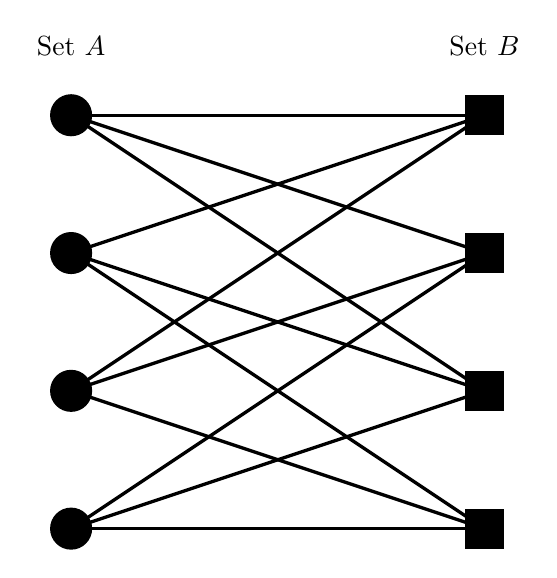
\begin{tikzpicture}[scale=1.75]

\node at (-1.5, 2) {Set $A$};
\node at (1.5, 2) {Set $B$};

\draw [fill=black,very thick] (-1.5,1.5) circle (4pt);
\draw [fill=black,very thick] (-1.5,0.5) circle (4pt);
\draw [fill=black,very thick] (-1.5,-0.5) circle (4pt);
\draw [fill=black,very thick] (-1.5,-1.5) circle (4pt);

\filldraw ([xshift=-4pt,yshift=-4pt]1.5,1.5) rectangle ++(8pt,8pt);
\filldraw ([xshift=-4pt,yshift=-4pt]1.5,0.5) rectangle ++(8pt,8pt);
\filldraw ([xshift=-4pt,yshift=-4pt]1.5,-0.5) rectangle ++(8pt,8pt);
\filldraw ([xshift=-4pt,yshift=-4pt]1.5,-1.5) rectangle ++(8pt,8pt);

\draw [very thick] (-1.5,1.5) -- (1.5,1.5);
\draw [very thick] (-1.5,1.5) -- (1.5,0.5);
\draw [very thick] (-1.5,1.5) -- (1.5,-0.5);

\draw [very thick] (-1.5,0.5) -- (1.5,-1.5);
\draw [very thick] (-1.5,0.5) -- (1.5,-0.5);
\draw [very thick] (-1.5,0.5) -- (1.5,1.5);

\draw [very thick] (-1.5,-0.5) -- (1.5,1.5);
\draw [very thick] (-1.5,-0.5) -- (1.5,-1.5);
\draw [very thick] (-1.5,-0.5) -- (1.5,0.5);

\draw [very thick] (-1.5,-1.5) -- (1.5,-0.5);
\draw [very thick] (-1.5,-1.5) -- (1.5,-1.5);
\draw [very thick] (-1.5,-1.5) -- (1.5,0.5);


\end{tikzpicture}
\caption{A random bipartite trivalent graph.}
\end{center}
\end{figure}
%%%%% END OF FIGURE %%%%%




%%%%% DOUBLE RING GRAPH %%%%%

\subsubsection{Double Ring Graph}

One ordered graph that will also be studied in the course of this project is the `double ring graph'. It is called this as the points can be visualised as two rings with one's centre directly above the other. Each have nodes uniformly spaced over their perimeter with the nodes on the bottom ring being connected to the nodes directly above them. each node is also connected to its two adjacent nodes on its ring. This graph is both trivalent and bipartite. Obviously, it is not considered to be random due to its very clear ordering pattern.

An alternative way of viewing the double ring graph is shown in figure FILL. The reason for representing the graph this way is that it is much easier to see all the nodes and connections on paper. Note that periodic boundary conditions are in place in this graph.

%%%%%%%%%%% DOUBLE RING PICTURE %%%%%%%%%%

\begin{figure}
\begin{center}
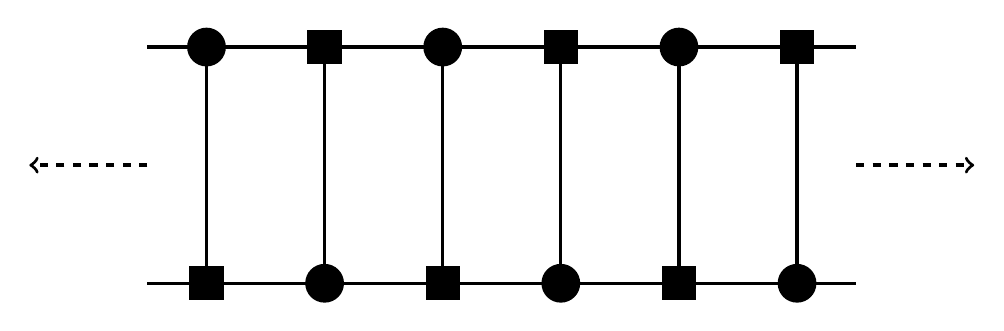
\begin{tikzpicture}[scale=1.5]

\draw [fill=black,very thick] (-2.5,1) circle (0.15cm);
\draw [fill=black,very thick] (-1.5,-1) circle (0.15cm);
\draw [fill=black,very thick] (-0.5,1) circle (0.15cm);
\draw [fill=black,very thick] (0.5,-1) circle (0.15cm);
\draw [fill=black,very thick] (1.5,1) circle (0.15cm);
\draw [fill=black,very thick] (2.5,-1) circle (0.15cm);

\filldraw ([xshift=-4pt,yshift=-4pt] -2.5,-1) rectangle ++(8pt,8pt);
\filldraw ([xshift=-4pt,yshift=-4pt] -1.5,1) rectangle ++(8pt,8pt);
\filldraw ([xshift=-4pt,yshift=-4pt] -0.5,-1) rectangle ++(8pt,8pt);
\filldraw ([xshift=-4pt,yshift=-4pt] 0.5,1) rectangle ++(8pt,8pt);
\filldraw ([xshift=-4pt,yshift=-4pt] 1.5,-1) rectangle ++(8pt,8pt);
\filldraw ([xshift=-4pt,yshift=-4pt] 2.5,1) rectangle ++(8pt,8pt);

\draw [very thick] (-3,1) -- (3,1);
\draw [very thick] (-3,-1) -- (3,-1);

\draw [very thick] (-2.5,1) -- (-2.5,-1);
\draw [very thick] (-2.5,1) -- (-1.5,1);

\draw [very thick] (-1.5,1) -- (-1.5,-1);
\draw [very thick] (-1.5,1) -- (-1.5,-1);

\draw [very thick] (-0.5,1) -- (-0.5,-1);
\draw [very thick] (-0.5,1) -- (-0.5,-1);

\draw [very thick] (0.5,1) -- (0.5,-1);
\draw [very thick] (0.5,1) -- (0.5,-1);

\draw [very thick] (1.5,1) -- (1.5,-1);
\draw [very thick] (1.5,1) -- (1.5,-1);

\draw [very thick] (2.5,1) -- (2.5,-1);
\draw [very thick] (2.5,1) -- (2.5,-1);

\draw [->][dashed, very thick] (3,0) to (4,0);
\draw [->][dashed, very thick] (-3,0) to (-4,0);

\end{tikzpicture}
\caption{Double ring bipartite graph. The circular nodes belong to set $A$ and the square nodes to set $B$. The dashed lines represent that the graph loops back around on itself and one end joins the other (periodic boundary conditions).}
\end{center}
\end{figure}

%%%%%%%%% END OF PIC %%%%%%%%%%%%%%



%%%%% OUTLINE OF PROBLEM %%%%%

\subsection{Outline of Problem}

The problem being considered during this project is that of assigning spin values ($\pm1$) to each node on the graph. The nodes that any given node interacts with is determined by the edges a node has. These are called a node's neighbours, and are essential in performing an update step on a node.

The aim is to run an Ising model simulation on a random bipartite graph structure. This is different to the regular Ising model simulation described above because of the randomness of the connection structure. In the `normal' version every subgrid (MPI process) only needs to be sent the values from the nearest edges of its neighbouring subgrids. This is due to the regularity of the grid structure.

This is not the case for a random graph. Nodes are neighboured with other nodes that are not `near' them and this neighbouring follows no pattern. This makes data division (how the graph is split between MPI processes) trickier and will also have a significant on the number of MPI sends and receives that will need to be performed. It will also mean that, most likely, more data will have to be sent in each MPI send than is need to be sent in the regular lattice configuration.

%%%%% MOTIVATION %%%%%

\subsection{Motivation}

The aim of this project is to solve ising model simulations on random, bipartite, trivalent graphs. The phase structure of such graphs will be examined, as will the software architecture and performance of MPI communications over a random graph structure.

%%%%% MPI %%%%%

\subsubsection{Why This Is An Interesting MPI Problem?}

This is an interesting problem from an MPI point of view because of the randomness of the graph. This makes the simulations much more communication heavy since it is more than likely that every MPI process will need to communicate with every other other MPI process between update steps. There is no pattern to how nodes are connected to each other and therefore the 

%%%%% PHYSICS %%%%%

\subsubsection{Physical uses of these simulations}

This problem is of interest in the field of physics as not much research has been done on the topic of spin models on random bipartite graphs. Spin models on regular lattice structures have been studied in detail for some time now, but there is very little on random graphs. It is interesting from a physics point of view to see the phase structures of such graphs.

%%%%% AIMS %%%%%
\subsection{Aims}

Since the begining of the porject the primary aim was to write a program that runs an Ising model simulation for a random, bipartite, trivalent graph, and to use this program to examine how the speed-up scales with an increase of core count and to examine the phase structure of such a graph.

The secondary aims of the project were:
\begin{enumerate}
\item To construct a `double ring' graph and run an ising model simulation on its topology. To examine the phase transition of this graph.
\item To determine the most efficient way to generate a random, bipartite, trivalent graph in both serial and parallel. To examine how such a method scales on multiple MPI cores. To explore how many steps it takes to make a graph is sufficiently random, and what the criteria should be for a graph to be considered random.
\item To generate random bipartite graphs that aren't trivalent (have more than three edges per node, or have a varying number of edges per node) and to run them on the simulation and examine the phase transition.
\item To find the most efficient method of organising random data to be sent between MPI processes.
\end{enumerate}

\newpage

%%%%%%%%%%%%%%%%%%%%%%%%%%%%%%%%%
%%%%% SOFTWARE ARCHITECTURE %%%%%
%%%%%%%%%%%%%%%%%%%%%%%%%%%%%%%%%

\section{Software Architecture}

In this section I will discuss the various techniques used in creating the simulations that were run in the duration of this project. The main areas these fall under are: graph generating - in both serial and parallel, as well as associated swap algorithms; MPI communication structure; and, finally, how the update step worked.

%%%%% RANDOM GRAPH GENERATION %%%%%
\subsection{Random graph generation}

Over the course of this project numerous different methods were implemented and compared for the `best' way to create a random bipartite graph. These methods were written in both serial and parallel.

%%%%% RANDOM GRAPHS IN SERIAL %%%%%
\subsubsection{Generating random graphs in serial}

There were two methods employed to generate random graphs over the course of this project. The first method (which we will call \emph{simple generation}) was mainl used in testing as it was not guaranteed to generated a connected graph once the number of nodes was increased over 40 (approximately). It also could not be generalised as easily to parallel code and is only applicable for generating bipartite, trivalent graphs. The second, and main, method is the swap algorithm which is discussed in detail in the following subsection.

For completeness the simple generation method is included here.

The simple generation method works by building the set of neighbours of one of the bipartite sets and then using that to reverse engineer the other. The first set, set $A$, is generated using the simple rules:

\begin{enumerate}
\item Each node in set $A$ must have exactly three unique neighbours.
\item In the set of all neighbours of $A$ each node index of nodes in $B$ must appear exactly three time.
\end{enumerate}

The first rule ensure that the graph is trivalent, from $A$'s point of view, with three unique nodes in $B$ as neighbours. The second rule ensures that each point in $B$ has three neighbours, as it only allows three points in $A$ to connect to each point in $B$.

This method is works quite well in serial, as it starts at node $0$ and fills in its neighbours and then continues all the way down to node $n-1$. The only complication is in filling in the final three nodes where some fairly simple checks must be preformed to ensure that the last three `slots' to fill in aren't `illegal' moves. By this, it is meant that filling the slots with the remaining available values would break one of the rules above.

%%%%% SWAP ALG %%%%%
\subsubsection{Swap algorithms in serial and parallel}

%%%%% SWAP ALG PIC %%%%%
\begin{figure}
\begin{center}
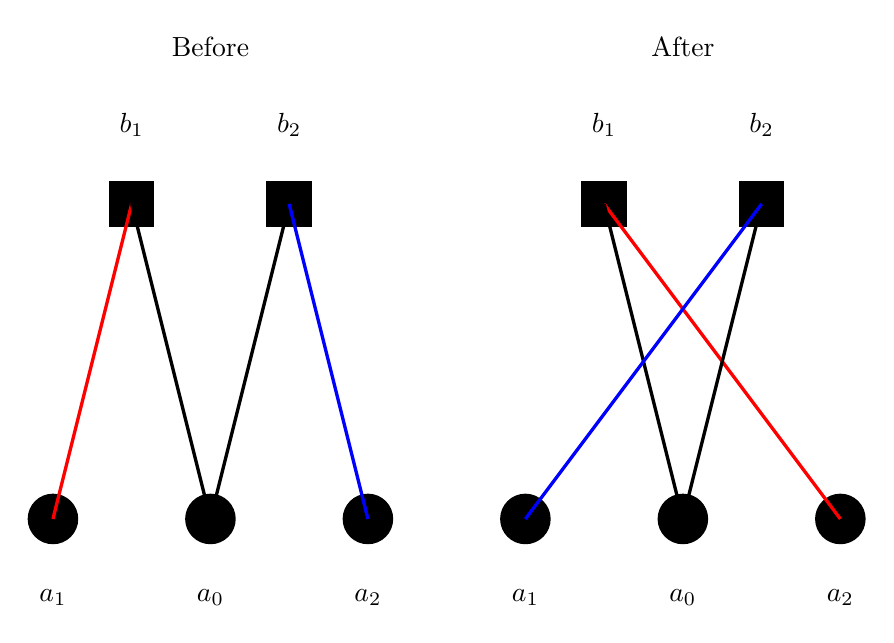
\begin{tikzpicture}[scale=2]

\draw [fill=black,very thick] (-2.5,-1) circle (0.15cm);
\node at (-2.5, -1.5) {$a_1$};
\draw [fill=black,very thick] (-1.5,-1) circle (0.15cm);
\node at (-1.5, -1.5) {$a_0$};
\draw [fill=black,very thick] (-0.5,-1) circle (0.15cm);
\node at (-0.5, -1.5) {$a_2$};

\filldraw ([xshift=-4pt,yshift=-4pt] -2,1) rectangle ++(8pt,8pt);
\node at (-2, 1.5) {$b_1$};
\filldraw ([xshift=-4pt,yshift=-4pt] -1,1) rectangle ++(8pt,8pt);
\node at (-1, 1.5) {$b_2$};

\draw [red, very thick] (-2.5,-1) -- (-2,1);
\draw [very thick] (-2,1) -- (-1.5,-1);
\draw [very thick] (-1.5,-1) -- (-1,1);
\draw [blue, very thick] (-1,1) -- (-0.5,-1);

\draw [fill=black,very thick] (2.5,-1) circle (0.15cm);
\node at (2.5, -1.5) {$a_2$};
\draw [fill=black,very thick] (1.5,-1) circle (0.15cm);
\node at (1.5, -1.5) {$a_0$};
\draw [fill=black,very thick] (0.5,-1) circle (0.15cm);
\node at (0.5, -1.5) {$a_1$};

\node at (-1.5, 2) {Before};
\node at (1.5, 2) {After};

\filldraw ([xshift=-4pt,yshift=-4pt] 2,1) rectangle ++(8pt,8pt);
\node at (2, 1.5) {$b_2$};
\filldraw ([xshift=-4pt,yshift=-4pt] 1,1) rectangle ++(8pt,8pt);
\node at (1, 1.5) {$b_1$};

\draw [red, very thick] (2.5,-1) -- (1,1);
\draw [very thick] (2,1) -- (1.5,-1);
\draw [very thick] (1.5,-1) -- (1,1);
\draw [blue, very thick] (0.5,-1) -- (2,1);

\end{tikzpicture}
\caption{Swap alg.}
\end{center}
\end{figure}

The swap aglorithm is used for two purposes in this project. The main use is in the generation of random graphs, and a secondary use is as a proposal step during an update (instead of proposing a spin flip a swap is proposed instead) MIGHT DO THIS COME BACK TO.

In the simplest terms the swap algorithm takes two points in one bipartite set and chooses a neighbour of each of the chosed points and then swaps the connectivity, so that the first point is now a neighbour to the point who was neighbouring the second point, and vice versa. The main advantage of using this swap algorithm is that it preserves the properties of the graph. If we start with a bipartite, trivalent graph and do 1000 swaps, say, then the graph will still remain bipartite and trivalent.

The algorithm preserves this because each swap ensures that points in set $A$ remain only connected to points in set $B$. It also does not change the number of edges coming out of any vertices, this is because it simply two edges are directly swapped with each other between pairs of points so all points involved retain the number of connections they have.

\paragraph{The algorithm} ~\\

The algorithm works by first choosing a node in set $A$, at random, which we will call $a_0$ . From this node two of its neighbours in set $B$ are chosen (again, at random), we call these $b_1$ and $b_2$. The next step is to choose one neighbour each of $b_1$ and $b_2$, ensuring not to choose $a_0$ again. Label the neighbour of $b_1$ as $a_1$ and the neighbour of $b_2$ as $a_2$. At this point we have the nodes selected that we wish to swap. We want to have $b_1$ not connected to $a_1$ anymore, but instead have it connected to $a_2$, and similarly no longer have $b_2$ connected to $a_2$, but connected to $a_1$.

Before we can do this however we must preform some checks. We must ensure that $a_1$ is not connected to $b_2$ by any other edge that we have not considered so far, and similarly we must must ensure that $a_2$ is in no way connected to $b_1$. The reason for this check is that we may already have the nodes we wish to swap connected to each other by another edge, so if the swap is performed then it would mean having two edges connecting the same two points to each other, which is not desirable.



\paragraph{Serial Implementation} ~\\

Implementing the algorithm in serial is a rather straightforward. It follows the description given above and there is no complication involving which point is hosted on which process. The hardest part of writing the code for this algorithm was doing the checks at the end to ensure that the points you were swapping weern't already neighbours through another edge that hadn't yet been considered.

\begin{breakablealgorithm}
\caption{Serial swap algorithm}
\begin{algorithmic}

\State Pick $a_0 =$ \verb|rand| $\in A$

\While {$b_1 \neq b_2$}
\State $b_1 =$ \verb|rand| $\in N(a_0)$
\State $b_2 =$ \verb|rand| $\in N(a_0)$
\EndWhile

\While {$flag = 1$}

\While {$a_1 \neq a_2$, $a_1 \neq a_0$, $a_2 \neq a_0$}
\State $a_1 =$ \verb|rand| $\in N(b_1)$
\State $a_2 =$ \verb|rand| $\in N(b_2)$
\EndWhile

\If {$a_1 \in N(b_2)$}
\State $flag =1$
\EndIf

\If {$a_2 \in N(b_1)$}
\State $flag =1$
\EndIf

\State Do swap:
\State $a_2 \in N(b_1)$ and $a_1 \in N(b_2)$
\State $b_2 \in N(a_1)$ and $b_1 \in N(a_2)$

\EndWhile

\end{algorithmic}
\end{breakablealgorithm}
%%%%%%%% END ALG %%%%%%%%

\paragraph{Parallel Implementation} ~\\

The parallel implementation of this algorithm is, naturally, a little more tricky. It is also a problem that does not parallise well at all. In fact, the serial algorithm is much faster and more efficient. The main reason for this is that in the parallel version nodes, and information about what connections they have, are stored on different processors. This means that every time it is needed to pick another node or check a node's neighbours every other processor must wait while one processor does the work. These tasks can't be done simultaneously during the algorithm since each step is directly dependent on the previous step. The problem also can't be avoided by running the algorithm twice (or more) at the same time. This is because, again the whole geometry of the graph must be know in order for the swap to happen, and if one version changes the graph then the other versions don't know about this change yet and so could make a swap that no longer exists on the graph.

%%%%%% PARALLEL SWAP ALG %%%%%%%

\begin{breakablealgorithm}
\caption{Parallel swap algorithm}
\begin{algorithmic}

\If {$rank = 0$}
\State Pick $a_0 =$ \verb|rand| $\in A$
\State Determine rank of proc $a_0$ is hosted on, $rank(a_0)$
\EndIf

\State \verb|MPI_Bcast(a_0,...,0,...)|
\State \verb|MPI_Bcast(rank(a_0),...,0,...)|

\If {$rank = rank(a_0)$} 
\While {$b_1 \neq b_2$}
\State $b_1 =$ \verb|rand| $\in N(a_0)$
\State $b_2 =$ \verb|rand| $\in N(a_0)$
\EndWhile
\EndIf

\State \verb|MPI_Bcast(b_1,...,rank(a_0),...)|
\State \verb|MPI_Bcast(b_2,...,rank(a_0),...)|

\State Determine rank of proc $b_1$ is hosted on, $rank(b_1)$
\State Determine rank of proc $b_2$ is hosted on, $rank(b_2)$

\While {$flag=1$}
\While {$a_1 \neq a_2$, $a_1 \neq a_0$, $a_2 \neq a_0$}
\If { $rank = rank(b_1)$}
\State $a_1 =$ \verb|rand| $\in N(b_1)$
\EndIf
\If{ $rank = rank(b_2)$}
\State $a_2 =$ \verb|rand| $\in N(b_2)$
\EndIf
\EndWhile

\If {$a_1 \in N(b_2)$}
\State $flag =1$
\EndIf

\If {$a_2 \in N(b_1)$}
\State $flag =1$
\EndIf

\EndWhile
\State \verb|MPI_Bcast(a_1,...,rank(b_1),...)|
\State \verb|MPI_Bcast(a_2,...,rank(b_2),...)|

\State Determine rank of proc $a_1$ is hosted on, $rank(a_1)$
\State Determine rank of proc $a_2$ is hosted on, $rank(a_2)$

\State Do swap:
\If {$rank = rank(a_1)$}
\State $b_2 \in N(a_1)$
\EndIf

\If {$rank = rank(a_2)$}
\State $b_1 \in N(a_2)$
\EndIf

\If {$rank = rank(b_1)$}
\State $a_2 \in N(b_1)$
\EndIf

\If {$rank = rank(b_2)$}
\State $a_1 \in N(b_2)$
\EndIf


\end{algorithmic}
\end{breakablealgorithm}

%%%%%%%% END OF ALG %%%%%%%%


%%%%% OVERVIEW OF PARALLEL SIMULATION %%%%%

\subsection{General Overview of Parallel Simulation}

In this section a general overview of how the code written for this project works. In the following sections some of the more complicated steps will be explained in greater detail.

The program is first initialised with MPI on the required number of processors, \verb|num_proc|. The number of nodes, \verb|num_nodes| in the graph to be solved is determined. Each bipartite set gets half of these points.

Two typedef'd struct called \verb|Array| is initialised on each CPU, one is for the nodes in set $A$, the other for the nodes in set $B$. This structure contains the total number of nodes in the set, the local number of nodes, the offset of the array and a list of all the neighbours of the nodes held localy.

\begin{lstlisting}
typedef struct
{
	int x; // global number of nodes in set
	int x_local; // local number of nodes in set
	int x_offset; // Array offsets
	int **neighbour; // array of neighbouring points
}
Array;
\end{lstlisting}

The element \verb|**neighbour| is a two dimensional array. Its size is determined at run-time by the size of the graph, number of processors and the number of neighbours each point has. The first index, $i$, is the local index of a node in the array, the second index, $j$, is the index of $i$'s $j^{th}$ neighbour. So if we have an array for set $A$ denoted simply by \verb|a| then \verb|a->neighbour[i][j]| gives the global index of the $j^{th}$ neighbour of $i$. $i$'s global index is given by: \verb|i_global = a->x_local*a->x_offset + i|.

The array is initialised into a double ring configuration by default. The reason for this is that it is very simple to set up. Each node's neighbours are simply the points with global indices $n-1$, $n$ and $n+1$ all in set $B$, if we are considering the node with global index $n$ in set $A$.


The next step is to run the swap algorithm, as described in the previous section, a sufficient number of times in order to randomise the graph.

A similar struct to \verb|Array|, called \verb|Field| is then initialised. Like the array struct it is initialised on ever processor twice, once for nodes in $A$ and once for $B$. This struct has three elements. The first is the value array. This is an array of length \verb|a->x_local|. It holds the value of the spin each node has. Spin is denoted as $\uparrow = +1$ and $\downarrow = -1$.

\begin{lstlisting}
typedef struct
{
	int *value;	// vals for points on local process
	int *halo_count; // no of points recived from each proc
	int **halo;	// vals of data recieved from each proc	
}
Field;
\end{lstlisting}

The \verb|*halo_count| array is the same size of the number of processors that the code is running on. It is a counter that measures how many data points will be sent from each other process to the host process. For example \verb|if(host.rank==0) f_a->halo_count[2] = 7| means that if the host process is rank 0, then it expects to be sent 7 data points from process 2.

Finally, the two dimensional array \verb|**halo| is the array that actually holds the values that are sent to the host process from the other processors. The first index of this array denotes the process from which the data is to be received from. The second index is the counter for the recieved data. Continuing with the example from the last paragraph, if we have \verb|if(host.rank==0) f_a->halo_count[2] = 7| then \verb|if(host.rank==0) f_a->halo[2][j]| has 7 elements, where $j$ determines which value is which, when the data is received.

The number of data points that need to be sent from each processor to every other processor is then computed (more on this method later). The next step is to malloc space for the points needed from other procs to be stored locally on the host proc.

At this point it is known on each processor how many nodes are needed from each of the other processes in order to complete an up date step. Before each update step is started, all the values that must be sent from one process to another must be completed. This sending of data requires loading the relevant values into a send buffer, sending them to their correct destination with an MPI call. These values are received into a receive buffer and are then copied into the the halo array of the field struct (all of this is explained in more detail further on). The update step then calls the values from this halo when they are needed.




%%%%% MPI %%%%%
\subsection{MPI communications}


%%%%% DATA DIVISION %%%%%
\subsubsection{Data division and load balancing}

The problem of how to split the data most efficiently between computing cores will be handled in this section. When we want to solve the system in parallel we have to give each processor a certain number of points on the graph. The method used to divide the data was to simply divide the nodes equally among the processors. This may seem, at first glance, as though it isn't the most efficient way to distribute the data in order to minimise the MPI communication overhead of the calculation. However, it is actually the fairest and easiest way to balance each processor's load and have a, relatively, uniform spread of MPI communications between processors.

This is the fairest method because if the graph is truly random it is expect that each processor needs to communicate with, on average, the same number of nodes on each of the other processors. This division then ensures that each processor sends the same (on average) data points from itself to each other processor.

The alternative to this method is to do some sort of profiling and then preconditioning of the graph and connections. The purpose of this would be to minimise the amount of data that needs to be sent between nodes. This would be a very complicated algorithm that would most likely require a lot of computation time. This large addtional overhead would greatly overshadow any of the benefits gained in the actual computation.


%%%%% DATA DIVISION PIC %%%%%
\begin{figure}
\begin{center}
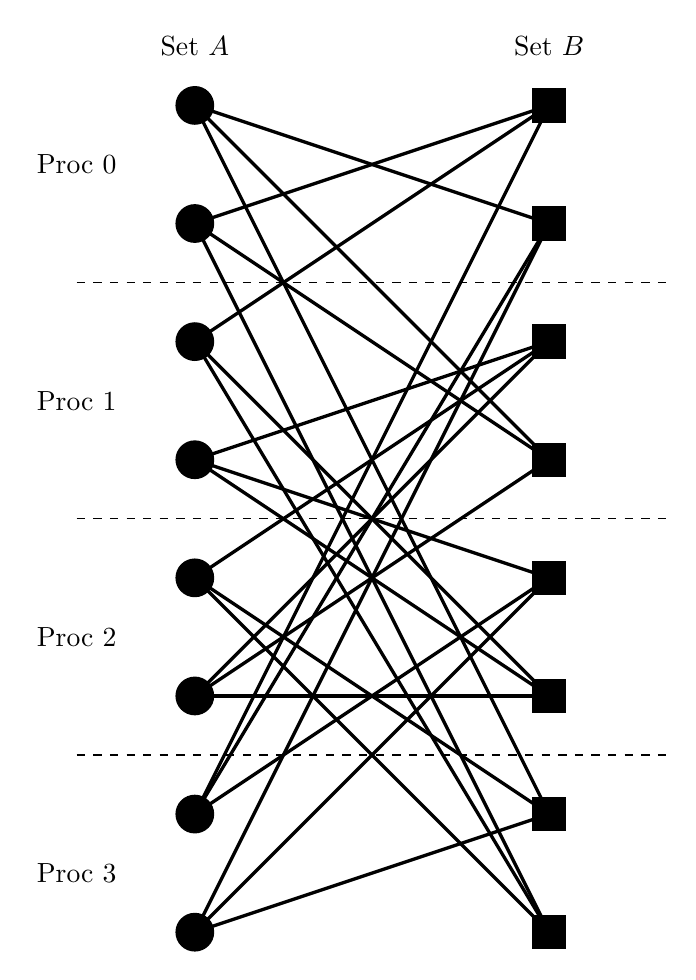
\begin{tikzpicture}[scale=1.5]


\node at (-1.5, 4) {Set $A$};
\node at (1.5, 4) {Set $B$};

\node at (-2.5, 3) {Proc $0$};
\node at (-2.5, 1) {Proc $1$};
\node at (-2.5, -1) {Proc $2$};
\node at (-2.5, -3) {Proc $3$};


\draw [fill=black,very thick] (-1.5,3.5) circle (0.15cm);
\draw [fill=black,very thick] (-1.5,2.5) circle (0.15cm);
\draw [fill=black,very thick] (-1.5,1.5) circle (0.15cm);
\draw [fill=black,very thick] (-1.5,0.5) circle (0.15cm);
\draw [fill=black,very thick] (-1.5,-0.5) circle (0.15cm);
\draw [fill=black,very thick] (-1.5,-1.5) circle (0.15cm);
\draw [fill=black,very thick] (-1.5,-2.5) circle (0.15cm);
\draw [fill=black,very thick] (-1.5,-3.5) circle (0.15cm);

\draw [dashed] (-2.5,2) -- (2.5,2);
\draw [dashed] (-2.5,0) -- (2.5,0);
\draw [dashed] (-2.5,-2) -- (2.5,-2);

\filldraw ([xshift=-4pt,yshift=-4pt]1.5,3.5) rectangle ++(8pt,8pt);
\filldraw ([xshift=-4pt,yshift=-4pt]1.5,2.5) rectangle ++(8pt,8pt);
\filldraw ([xshift=-4pt,yshift=-4pt]1.5,1.5) rectangle ++(8pt,8pt);
\filldraw ([xshift=-4pt,yshift=-4pt]1.5,0.5) rectangle ++(8pt,8pt);
\filldraw ([xshift=-4pt,yshift=-4pt]1.5,-0.5) rectangle ++(8pt,8pt);
\filldraw ([xshift=-4pt,yshift=-4pt]1.5,-1.5) rectangle ++(8pt,8pt);
\filldraw ([xshift=-4pt,yshift=-4pt]1.5,-2.5) rectangle ++(8pt,8pt);
\filldraw ([xshift=-4pt,yshift=-4pt]1.5,-3.5) rectangle ++(8pt,8pt);

\draw [very thick] (-1.5,3.5) -- (1.5,2.5);
\draw [very thick] (-1.5,3.5) -- (1.5,0.5);
\draw [very thick] (-1.5,3.5) -- (1.5,-2.5);

\draw [very thick] (-1.5,2.5) -- (1.5,3.5);
\draw [very thick] (-1.5,2.5) -- (1.5,0.5);
\draw [very thick] (-1.5,2.5) -- (1.5,-3.5);

\draw [very thick] (-1.5,1.5) -- (1.5,-3.5);
\draw [very thick] (-1.5,1.5) -- (1.5,3.5);
\draw [very thick] (-1.5,1.5) -- (1.5,-1.5);

\draw [very thick] (-1.5,0.5) -- (1.5,-1.5);
\draw [very thick] (-1.5,0.5) -- (1.5,-0.5);
\draw [very thick] (-1.5,0.5) -- (1.5,1.5);

\draw [very thick] (-1.5,-0.5) -- (1.5,1.5);
\draw [very thick] (-1.5,-0.5) -- (1.5,-2.5);
\draw [very thick] (-1.5,-0.5) -- (1.5,-3.5);

\draw [very thick] (-1.5,-1.5) -- (1.5,-1.5);
\draw [very thick] (-1.5,-1.5) -- (1.5,1.5);
\draw [very thick] (-1.5,-1.5) -- (1.5,0.5);

\draw [very thick] (-1.5,-2.5) -- (1.5,-0.5);
\draw [very thick] (-1.5,-2.5) -- (1.5,3.5);
\draw [very thick] (-1.5,-2.5) -- (1.5,2.5);

\draw [very thick] (-1.5,-3.5) -- (1.5,-0.5);
\draw [very thick] (-1.5,-3.5) -- (1.5,-2.5);
\draw [very thick] (-1.5,-3.5) -- (1.5,2.5);

\end{tikzpicture}
\caption{Data division for a random trivalent, bipartite graph.}
\end{center}
\end{figure}

%%%%%%%%%%%%% END OF PIC %%%%%%%%%%%%%%




%%%%% SETTING UP HALO REGIONS %%%%%

\subsubsection{Setting up Halo Regions}

To understand why the halo region is needed and how it works, it is easiest to use a picture. Consider the graph shown in figure FILL. It shows two bipartite sets each with six nodes. The graph is divided over three processors. We are going to consider performing an update on the nodes in set $A$ hosted on processor 1. The figure only shows the edges that connect the nodes in set $A$ on process 1 to nodes that are not on process 1. All other nodes are not shown as they aren't necessary in understanding the method.

%%%%% SET UP HALO PICTURE %%%%%
\begin{figure}
\begin{center}
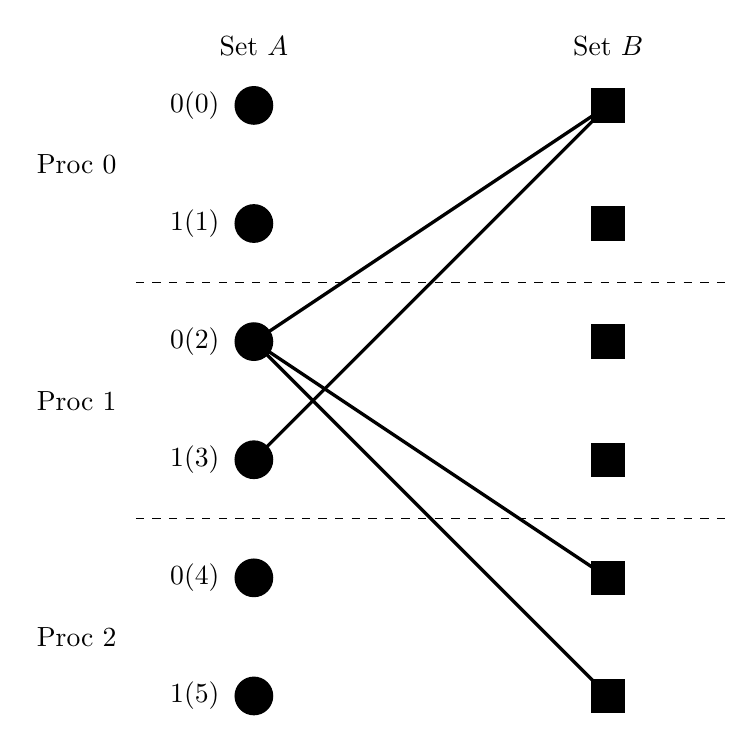
\begin{tikzpicture}[scale=1.5]

\node at (-1.5, 3) {Set $A$};
\node at (1.5, 3) {Set $B$};

\node at (-3, 2) {Proc $0$};
\node at (-3, 0) {Proc $1$};
\node at (-3, -2) {Proc $2$};

\node at (-2, 2.5) {$0 (0)$};
\node at (-2, 1.5) {$1 (1)$};
\node at (-2, 0.5) {$0 (2)$};
\node at (-2, -0.5) {$1 (3)$};
\node at (-2, -1.5) {$0 (4)$};
\node at (-2, -2.5) {$1 (5)$};

\draw [fill=black,very thick] (-1.5,2.5) circle (0.15cm);
\draw [fill=black,very thick] (-1.5,1.5) circle (0.15cm);
\draw [fill=black,very thick] (-1.5,0.5) circle (0.15cm);
\draw [fill=black,very thick] (-1.5,-0.5) circle (0.15cm);
\draw [fill=black,very thick] (-1.5,-1.5) circle (0.15cm);
\draw [fill=black,very thick] (-1.5,-2.5) circle (0.15cm);

\draw [dashed] (-2.5,1) -- (2.5,1);
\draw [dashed] (-2.5,-1) -- (2.5,-1);

\filldraw ([xshift=-4pt,yshift=-4pt]1.5,2.5) rectangle ++(8pt,8pt);
\filldraw ([xshift=-4pt,yshift=-4pt]1.5,1.5) rectangle ++(8pt,8pt);
\filldraw ([xshift=-4pt,yshift=-4pt]1.5,0.5) rectangle ++(8pt,8pt);
\filldraw ([xshift=-4pt,yshift=-4pt]1.5,-0.5) rectangle ++(8pt,8pt);
\filldraw ([xshift=-4pt,yshift=-4pt]1.5,-1.5) rectangle ++(8pt,8pt);
\filldraw ([xshift=-4pt,yshift=-4pt]1.5,-2.5) rectangle ++(8pt,8pt);


\draw [very thick] (-1.5,0.5) -- (1.5,2.5);
\draw [very thick] (-1.5,-0.5) -- (1.5,2.5);

\draw [very thick] (-1.5,0.5) -- (1.5,-1.5);
\draw [very thick] (-1.5,0.5) -- (1.5,-2.5);

\end{tikzpicture}
\caption{FILL}
\end{center}
\end{figure}
%%%%% END HALO PICTURE %%%%%

We start by looking at the nodes in set $A$, on process 1, and where this data is needed. First we looping over the array of neighbours of nodes in set $A$. First the neighbours of point 0 (global index 2) are examined. It has neighbours 0, 4 and 5 (global indices). Point 0 is on process 0, and points 4 and 5 are on process 2. So at this stage, on process 1 we know that \verb|send_count[0]=1| and \verb|send_count[2]=1|.

Since point 0 is connected to both 4 and 5 in set $B$ we have a double count which has to be ignored. Once we know that we need to send a point's data to another proc it is marked that it is needed and will not be sent again. To keep track of double counts like this we need a two dimensional array \verb|**double count|. The first index is for the local index of a node and the second is for the process that the data is to be sent to. So for node 0 on process 1 we have \verb|double_count[0][2]=1|. Initially this is value is zero to say that point is not needed on process 1, but when we find that point 4 needs that value we set the double count entry to 1 to mark the value as counted for. So then when the program realises that point 5 also needs point 0 from process 1 we do not need to copy it again because we have marked it as copied already.

Then point 1 is looked at. Its only connection to another process is to point 0 (global index). Point zero is on process 0 and we have that \verb|double_count[1][0]=0| so we are free to increase the send count to process 0: \verb|send_count[0]=2|.

That is all the neighbours looped over and we know how many points process 0 has to send to each other process. Importantly, there has been no double counting, while it may not have been a big deal in this small example, but for a bigger graph it could mean allocating space for thousands more data points and then performing MPI calls for all of the double counted values. This would add up very quickly over the course of a big simulation and lead to an unnecessarily large MPI communication overhead that would have a big performance impact.

Below is the code snippet for this procedure.


\begin{lstlisting}
	for(i=0;i<a->x_local;i++){
		for(j=0;j<3;j++){
		proc = a->neighbour[i][j]/a->x_local;
			if(double_count[i][proc] == 0){
				// determine if neighbour is on a different proc
				if(a->neighbour[i][j] < host.rank*a->x_local || a->neighbour[i][j] >= (host.rank+1)*a->x_local){
					send_count[proc]++; // increase count if on diff proc
					double_count[i][proc] = 1;
				}
			}
		}
	}
\end{lstlisting}


At this stage it is known on process 1 how many of its local data points need to be sent to other processors. However, the other processors do not yet know how much data they will be receiving from every other process. For example process 0 does not yet know that it will be 2 data points from process 1. The recevie count array for each process tell it how many data points will be received from each other process. For example, on process 0 \verb|recv_count[1]| holds the number of data points that are to be received from process 1. These receive counts should match the send counts on the sending process with the destination process as the index. So on process 1 \verb|send_count[0]=2|, therefore we must have \verb|recv_count[1]=2| on process 0.

Instead of doing some sort of similar counting algorithm as was done to find the send count, it is much easier to use the \verb|MPI_Alltoall| command. This command will send take an array in the send buffer and a send count, $x$. It then sends the first $x$ elements of the array to process 0 the second $x$ to process 1 and so on. A receive count is also specified with a receive buffer telling the program what to do with the received data.

\begin{lstlisting}
	MPI_Alltoall(send_count, 1, MPI_INT, recv_count, 1, MPI_INT, MPI_COMM_WORLD);
\end{lstlisting}

Now that each processor knows how many data points it will receive from every other process the memory can be allocated to store this incoming data:

\begin{lstlisting}
	for(i=0;i<num_proc;i++)
		f_a->halo_count[i] = recv_count[i];

	f_a->halo = (int**)malloc(sizeof(int *)*host.np);

	for(i=0;i<num_proc;i++){
		if(f_a->halo_count[i] != 0){
			f_a->halo[i] = (int*)malloc(sizeof(int)*f_a->halo_count[i]);
		} else {
			f_a->halo[i] = NULL;
		}
	}
\end{lstlisting}


%%%%% SENDING DATA BETWEEN PROCESSORS %%%%%

\subsubsection{Sending Data Between Processors}

Now that the space for the data to be sent to has been allocated on each process, we can now load the data points into the relevant send buffer, send it, receive it and unpack it into the space we allocated in the previous section. This is implemented through a set of communicator functions for each stage described above.

The first part of this implementation is defining a typedef'd struct called \verb|BoundaryComm|. This will be initialised on each processor and hold:  the send and receive counts to/from each other processor, the send and receive buffers for storing the data to be sent/once it's received, and the double count array that works as before to avoid the over sending of data points. 

\begin{lstlisting}
typedef struct {
	int *send_count;
	int *recv_count;
	int **buffer_send;
	int **buffer_recv;
	int **double_count;
} BoundaryComm; 
\end{lstlisting}

The \verb|init_comm| function initialises the boundary communicator on each process and sets values for the send and receive counts. This is done using the exact same method as before when the halo space was initialised, with the doubele count array taking care of points being double counted as before. The send and receive counts are then used to malloc the send and receive buffers.

The \verb|send| function is the function responsible for loading the relevant data into the send buffer, sending the data to the correct process and receiving the data into the receive buffer. On each process, the neighbours of the points hosted on that process are looped over, as before. This time though it is ensured that each point to be loaded into the send buffer has the following condition met: \verb|c->double_count[point][proc]=1|. This is because, previously it was only points that were to be sent got this flag in their entry of the double count array. Once a point has been loaded to the buffer this value is set back to 0 so that it can't be loaded twice. It is simply to ensure that only the points that need to be sent are loaded into the buffer. The loop that carries out this operation is:

\begin{lstlisting}
for(i=0;i<a->x_local;i++){
		for(j=0;j<3;j++){
			proc = a->neighbour[i][j]/a->x_local;
			if(c->double_count[i][proc] == 1 ){
					// copy value into buffer
					if(f_a->value[i] == -1){
						val = 0;
					} else {
						val = 1;
					}
					c->buffer_send[proc][k[proc]] = 2*i + val;
					k[proc]++; // increase relavant buff index
					c->double_count[i][proc] = 0; // mark as loaded to buff
				}
			}
		}
\end{lstlisting} 

There is a slight problem with loading the values in to the buffer: the values will be loaded in a random order that is determined by to the order in which the neighbours appear on the array of neighbours. When it is then unpacked by a different processor this order remains. However running the same loop on the receiving process may (actaully, most certainly will for large random graphs) require the data to read out in a different order than it was fed in. For this reason a simple `first-in-first-out' method will not work. The most basic solution would be to send both the global index of a point with its spin value. However this doubles the already large amount of data that has to be sent. Instead it is more efficient to encode the index of the node \emph{and} its spin value into one \verb|int|.

This is done by simply doubling the value of the local index and adding 1 if it is spin up and not adding anything if it is spin down. This way when the data is received this small algorithm is simply reversed to give the spin and the node from where the data originated.

The data is sent and received using the non-blocking MPI calls \verb|MPI_Isend| and \verb|MPI_Irecv|. 

\begin{lstlisting}
	for(i=0;i<num_proc;i++){
		if(host.rank !=i){
			MPI_Isend((c->buffer_send[i]), c->send_count[i], MPI_INT, i, 100*host.rank, MPI_COMM_WORLD, send_ptr);
			send_ptr++;
			MPI_Irecv((c->buffer_recv[i]), c->recv_count[i], MPI_INT, i, 100*i, MPI_COMM_WORLD, recv_ptr);
			recv_ptr++;
		}
	}
	MPI_Waitall(host.np-1, send, send_status);
	MPI_Waitall(host.np-1, recv, recv_status);
\end{lstlisting}

At this stage the data has been sucessfully sent to the receiving processes and is ready to be unpacked into the the halo array that was created earlier. This simply involves the copying of the data into the halo:

\begin{lstlisting}
for(i=0;i<host.np;i++)
	for(j=0;j<c->recv_count[i];j++)
		f_a->halo[i][j] = c->buffer_recv[i][j];
\end{lstlisting}

The reversing of the encoding used to send the data is done later when the  data is actually needed for the update. The reason for not doing the decoding now is that then both the node and the spin need to be stored seperately in such a way that would allow easy access. However this is actually a hard procedure to implement and would save very little time in the computation. The algorithm for decoding the data is:

\begin{lstlisting}
for(i=0;i<a->x_local;i++){
	for(j=0;j<3;j++){
		// determine if neighbour is local or on another proc
		if(a->neighbour[i][j] < host.rank*a->x_local || a->neighbour[i][j] >= (host.rank+1)*a->x_local){
			k=0; 	
			proc = a->neighbour[i][j]/a->x_local; // rank of proc
			while(f_b->halo[proc][k]/2 != a->neighbour[i][j]%a->x_local){
				k++; // increment index until right point is found
			}
			val = f_b->halo[proc][k]%2;
			if( val == 0){
				spin[j] = -1;
			} else {
				spin[j] = 1;
			}
		} else { 
			spin[j] = f_b->value[a->neighbour[i][j]%a->x_local];
		}
	}
}
\end{lstlisting}

The processor a point belongs to is calculated by dividing the point's global index by the number of points per process, \verb|a->x_local|. The local index is given by the global index modulo the number of points per process. 

%%%%% PROBLEMS ENCOUNTERED IN IMPLEMENTATION %%%%%






\newpage
%%%%%%%%%%%%%%%%%%%
%%%%% RESULTS %%%%%
%%%%%%%%%%%%%%%%%%%

\section{Results and Analysis}

The results obtained over the course of this project are discussed in this section.

\subsection{Physics Results}

The aim of this project from a physics point of view was to explore whether or not spontaneous magnetisation occurs below a certain temperature for a random bipartite graph. This was done by running the simulation for a number of different values of $\beta$ where $\beta = \frac{1}{k_B T}$. So if there is an increase in $\beta$ it means that there is a decrease in temperature.

\subsubsection{Double Ring Graph}

The results for the double ring graph with 6400 nodes is shown in figure FILL. The simulation was run for $\beta$ varying from 0.05 to 3 in increments of 0.05. 50,000 update steps were performed at each value of $\beta$. The simulation That this graph came from was one that was run on 4 MPI processes. This simulation was also ran many other times on with many other values of the following parameters: number of processes, $\beta$ range, size of $\beta$ increments, number of update steps and the number of nodes on the graph. 

\begin{figure}
\centering
\includegraphics[scale=0.8]{double_ring_mag.jpg}
\caption{Double ring magnetisation}
\end{figure}

\subsubsection{Random Bipartite Trivalent graph}

\begin{figure}
\centering
\includegraphics[scale=0.8]{rand_mag.jpg}
\caption{Random graph magnetisation}
\end{figure}

\subsubsection{Serial}



%%%%% CODE PERFORMANCE RESULTS %%%%%

\subsection{Code Performance Results}

One of the central aims of this project was to determine how well the code performed. Timing data was collected for the solver on both random, bipartite, trivalent graphs and the double ring graph. These will be compared against each other and also compared against the scaling of similar code that solves the regular Ising model on the lattice.

In addition to this scaling data, the speed up of the parallel swapping algorithm will also be investigated

%%%%% SPEED UP RESULTS %%%%%%

\subsubsection{Speed Up Results}

The speed up of the solver was measured for both the double ring graph and the random graph. The speed up of the parallel swapping algorithm was also investigated. All are discussed in more detail in the subsections below.

\paragraph{Double Ring Graph} ~\\

To generate this speed up data for the double ring graph the simulation was run with 128,000 nodes for 50,000 update steps. The simulation was run on the Lonsdale cluster on 1, 2, 4, 8, 16, 32 and 64 MPI processes.

From the graph it is clear that the scaling is very good up until 32 processes (approximately linear scaling up to 16 cores). At 32 processes the speed up is 8.325 faster than the serial, and on 64 cores it drops further to 3.622 times faster than the serial version.

%%%%% SPEED UP PIC %%%%%
\begin{figure}
\centering
\includegraphics[scale=0.8]{d_r_speed.jpg}
\caption{Double ring speed up for a graph with 128,000 nodes and 50,000 update steps.}
\end{figure}
%%%%% END OF PIC %%%%%


\paragraph{Random Graph} ~\\

The speed up results for the random graph simulation can be seen in figure FILL. The graph used in the simulation had 32,768 nodes (16,384 per set). These were initialised in a double ring configuration before randomising the graph by calling the swap algorithm 88,4736 times. 50,000 update steps were performed. The simulation was run on Lonsdale for 1, 2, 4, 8, 16, 32 and 64 MPI processes. 

%%%%% SPEED UP PIC %%%%%
\begin{figure}
\centering
\includegraphics[scale=0.8]{rand_speed.jpg}
\caption{Random graph speed up}
\end{figure}
%%%%% END OF PIC %%%%%

Examining the graph we can see that overall the scaling is quite poor. The code runs nearly ten times slower on two cores than it does on one, and twice as slowly on four cores than the serial version (`speed up' for two cores is 0.121, and 0.490 for four). The code runs better on 8 and 16 cores (speed up of 2.820 and 3.342 respectively). 

\paragraph{Comparison to Ising Model on Regular Lattice} ~\\

The code used for this simulation was written by my supervisor, Professor Mike Peardon, for the Parallel Numerical Algorithms module he taught, and is available on his webpage.

%%%%% SPEED UP PIC %%%%%
\begin{figure}
\centering
\includegraphics[scale=0.8]{ising_graph.jpg}
\caption{This is the speed up graph of the Ising model on a regular lattice ($1024 \times 1024$).}
\end{figure}
%%%%% END OF PIC %%%%%


%%%%% SPEED UP COMPARISON PIC %%%%%
\begin{figure}
\centering
\includegraphics[scale=0.8]{comp.jpg}
\caption{Speed up comparison}
\end{figure}
%%%%%% END PIC %%%%%%


\subsubsection{Swap Algorithm}

In this section the performance of the swap algorithm is analysed. The serial version of the algorithm will be compared to the parallel algorithm for a varying number of cores. The number of swaps required to make a graph random will also be studied.



Before a graph is randomised for a simulation it is first initialised in an order that is fast and easy to compute. This is normally just the double ring cofiguration, where ever node has neighbours of the node with the same index, one ahead and one behind in the other bipartite set. From this initialisation we have to randomise the graph using the swap algorithm.

The problem here is knowing how many swaps need to be made before all traces of this original configuration are lost and the graph can be considered random. We know that initially every points neighbours are the three closest to it in our indexing system. So, if we have point $n$ in $A$ we know that its neighbours are $n-1$, $n$ and $n+1$ in set $B$.

If a graph is truly random then it is expected that given any node in set $A$, the probability of it being connected to any given node in $B$ is simply $\frac{1}{n_B}$, where $n_B$ is the number of nodes in $B$. So this means that if we divide the graph in half horizontally, as in the data division figure, we would expect, on average, half of our connections to cross this horizontal line.

In other words, if we think of how we divide a graph amongst processors by giving each processor an equar fraction of the nodes, we would then expect each processor to have the same, on average, connections to each other processor. This is easiest to think of with an example. Say we have a bipartite, trivalent graph where $n_A = n_B = 1024$, so there are $2048$ nodes in total. As each node in $A$ has three edges connecting it to nodes in $B$, the total number of edges in the graph is $3 \times 1024 = 3072$. If the graph is then divided by $4$ processors, then there are $\frac{3072}{4} = 768$ edges on each process.

Now, it is expected at this stage that the graph is random, therefore each of these $768$ edges on a process is equally likley to be on any of the $4$ processors. So we expect $\frac{768}{4} = 192$ connections on each process.

Code was written to simulate the exact situation described above and to determine how many swaps it takes to reach a random graph with no trace of its initial configuration.

\begin{figure}
\centering
\includegraphics[scale=0.8]{swap_random_1024_by_2_nodegraph.jpg}
\caption{This plot shows how the number of connections to different processors changes with the number of swaps performed. The graph used was a bipartite, trivalent graph with 1024 nodes in each set (2048 nodes in total). It was run on both 2 (green line) and 4 (red line) processors.}
\end{figure}


While the last simulation is useful for generating random graphs, it is also interesting, and possibly more useful, to examine how many swaps per node it takes for a graph to be considered random. This is interesting as this may be different for different sized graphs. To investigate this, the same simulation as above was run for varying graph sizes and a similar plot was made.

\begin{figure}
\centering
\includegraphics[scale=0.6]{swaps_per_node.jpg}
\caption{This plot shows how the average number of connections to another processor changes with the number of swaps performed per node. The graph used was a bipartite, trivalent graph with four different graph sizes (1024, 2048, 4096 and 8192). All were run on 4 processors.}
\end{figure}



\begin{figure}
\centering
\includegraphics[scale=0.8]{swap_speed.jpg}
\caption{Speed up of the swap algorithm.}
\end{figure}



%%%%% DOUBLE RING SPEED UP %%%%%

\subsubsection{Double Ring Graph}


\subsubsection{Random Graph}


\subsubsection{Swap Algorithm}

\subsection{How}

\newpage
%%%%%%%%%%%%%%%%%%%%%%
%%%%% CONCLUSION %%%%%
%%%%%%%%%%%%%%%%%%%%%%

\section{Conclusion}

hello

\newpage
%%%%%%%%%%%%%%%%%%%%%%%
%%%%% FUTURE WORK %%%%%
%%%%%%%%%%%%%%%%%%%%%%%

\section{Future Work}

There are a few things that I would like to have looked into during the course of this project but was not able to due to time constraints (a bug in my code had me stuck for weeks and I was not able to continue until it was fixed). Some areas that I think would be interesting in looking into are:
\begin{enumerate}
\item Running simulations on different types of graphs. It would be interesting to see the phase structure of graphs with more edges on each node or where not all nodes have the same number of edges connected to them. There is a small bit of tweaking that would have to be made to the structure of my code but it should be able to run such a simulation.
\item Using the swap algorithm as a proposal step in the update function. Perhaps instead of proposing a spin flip, a random swap of edges on the graph could be made. This would require a lot more thought than the previous point on how to implement sensibly, because if this is proposed the effects are much more wide reaching than one spin flip. It would be a difficult problem that probably requires a lot of thought but it would be interesting to see the result, if any.
\end{enumerate}

\newpage
\section{References}

\begin{enumerate}
\item Graph theory book by person
\item
\end{enumerate}

\end{document}
